
\emph{Slogan: clocks are an abstraction of threads?
  It's easier to manipulate, users can't make mistakes\ldots almost.
  We currently don't say anything about the (high-level) implementation.
  We can re-use most of the documentation on clocks here,
  notably illustrating the use of internal and external clocks.}

% <MOVED> DB The following has been moved from earlier sections

The timing, or clock, associated to a multimedia stream can be real-time, if the stream is created 
\TODO{DB scaled?}
or broadcasted live, or any scaled timing, for instance if the stream consists of files. \textit{A priori},
describing and broadcasting a stream implies real-time output. As we see later, this is unfortunately 
not sufficient for complex settings.
\TODO{DB infinite <> infallible}
Also, a stream can be finite or infinite. Infinite streams are particularly interesting for broadcasting
because most of the time, we expect a radio, for instance, to be always online. However, this needs 
a special care since it implies some assumption about the validity of the elements that build the stream.

\TODO{DB the following should move later}
Also, the stream generator can be used at any rate. For instance,
for a live broadcast, the generator will be asked to fill frames at real rate, while 
for a stream saved to a file, the generator will be asked to fill frames at the maximal possible rate.
\TODO{DB in the following, confusion between transition and crossing}

% </MOVED> DB 

Another limitation of the current model is the possibility to describe advanced transitions in 
the stream. For instance, one may want to use a crossfade between two tracks 
of the stream, \ie{}
fade out the volume of an ending track, fade in the volume of a starting track and merge this together.

\begin{figure}[t]
 \begin{center}
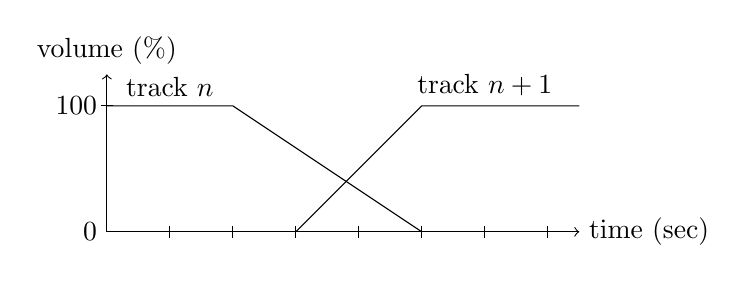
\begin{tikzpicture}[xscale=0.8,yscale=0.8]
\draw[->] (0,0) -- (0,2.5);
\draw (-0.1,2) -- (0.1,2);
\draw (0,2) node[anchor=east]{100};
\draw (0,0) node[anchor=east]{0};
\draw[->] (0,0) -- (7.5,0);
\foreach \x in {1,2,3,4,5,6,7} \draw (\x,-0.1) -- (\x,0.1);
\draw (0,2.5) node[anchor=south]{volume (\%)};
\draw (7.5,0) node[anchor=west]{time (sec)};
\draw (0,2) -- (2,2) -- (5,0);
\draw (3,0) -- (5,2) -- (7.5,2);
\draw (1,2) node[anchor=south]{track $n$};
\draw (6,2) node[anchor=south]{track $n+1$};
\end{tikzpicture}
\end{center}
 \caption{A crossfade transition between two tracks}
 \label{cross-fig}
 % Stream.png: 500x132 pixel, 91dpi, 14.03x3.70 cm, bb=0 0 398 105
\end{figure}

The initial source can be created, for instance, with a playlist of files. Then,
a \texttt{crossfade} operator would take this source and return a source whose tracks are 
crossfaded as shown in Figure \ref{cross-fig}. In order to do this, the operators has to 
detect sufficiently in advance the end of the current track, collect the data of the
end of the track, collect the data of the beginning of the next track, apply the respective
fade out and fade in and add the two streams to create the transition.

However, in this case we need to introduce a new notion in the model. Without transitions, the 
source generator can be used with a uniform rate on all nodes: frames are filled
at the same rate on every node. Unfortunately, the \texttt{crossfade} operator
does not have this property: when it detects the end of a track, it will query many frames in advance 
to the underlying source in order to compute the crossfade. This behaviour breaks the uniformity of 
timing in the graph and requires to introduce \textit{multiple clocks}.


\begin{figure}[b]
 \begin{center}
\[
\def\f{\save
*+<15pt>[F--]\frm{}\ar @{--} "2,2"\restore}%
\def\g{\save
"2,4"."1,2"."1,5"!C*+<27pt>[F--]\frm{}\ar @{--} "1,1"\restore}%
\xymatrix{
   \mathtt{clock_1} & *+[F]{\mathtt{playlist}}\ar[r]\f&*+[F]{\mathtt{crossfade}}\ar[r]&  *+[F]{\mathtt{fallback}}\ar[r]&
  *+[F]{\mathtt{output.icecast}}\\
   &\mathtt{clock_2} &  & *+[F]{\mathtt{jingles}}\ar[u]\g& 
}
\]
\end{center}
 \caption{A stream generator with different clocks}
 % Stream.png: 500x132 pixel, 91dpi, 14.03x3.70 cm, bb=0 0 398 105
\end{figure}

Clocks are represented in the model by a notion of locality in the graph. The graph is then partitioned into 
different sets, where each set shares the same clock.
When instantiating the graph, each operator declares if it needs a custom clock for him or its sources. 
Then, when initializing the graph of the stream generator, the clocks are attributed by a constraint 
satisfaction algorithm. Because of caching, we do not want a source to be connected to two different operators with 
two different clocks. In this case, this is detected when instantiating the graph and an error is raised.
Similarly, some sources do not support clocks whose rate is different than real time, for instance input 
from the local sound card. In this case too, if the clock attached to the source is not real time, an error
is raised.

